\documentclass[a4paper, 12pt]{article}

\usepackage[ngerman]{babel}
\usepackage[T1]{fontenc}
\usepackage{amsmath}
\usepackage{graphicx}
\usepackage[utf8]{inputenc}

\usepackage[a4paper,
            bindingoffset=0.2in,
            left=1cm,
            right=1cm,
            top=1in,
            bottom=1in,
            footskip=.25in]{geometry}
            
\title{Pre-LAB: Wärmekapazität, Team 4}
\author{Justus Weyers, Milena Mensching}

\begin{document}
\maketitle
\section{Größe eines Wassermoleküls}
\textbf{Wie groß ist ein Wassermolekül und wie viele Größenordnungen liegen zwischen ihm und einem Polystyrolpartikel mit einem Radius von $1\mu m$?}

Ein Wassermolekül ist ca. $0,3 nm$ groß. Der Durchmesser des Polystyrolpartikels liegt bei $2\mu m$. Anders ausgedrückt ist das Wassermolekül also $3 \cdot 10^{-10}m$ groß, während das Polystyrolpartikel $2* \cdot 10^{-6}m$  groß ist. Beide Größen trennen 4 dezimale Größenordnungen.

\section{Wie bewegen sich zwei kugelförmige Körper nach einem Stoß, wenn ihre Massen sehr
unterschiedlich sind und der schwere Körper ruht?}

Wenn $m_1>>m_2$, $v_1= 0 \frac{m}{s} $ und der zweite Körper sich mit einer Geschwindigkeit $v_2$ fortbewegt, handelt es sich bei einem Zusammenstoß der beiden Körper um einen zentralen elastischen Stoß. Der leichtere Körper mit der Masse $m_2$ prallt dabei in genau umgekehrter Richtung am schwereren Körper ab. Die Geschwindigkeit des leichteren Körpers ändert sich im Rahmen der Näherung und im Vergleich zur Richtung nicht: $v_2`= -v_2$. Bei einem elastischen Stoß wird keine kinetische Energie in innere Energie umgewandelt. Der Energie- und der Impulserhaltungsatz werden eingehalten.  

\section{Was ist eine Normalverteilung/Gaußverteilung? Was beschreiben ihr Mittelwert und ihre
Standardabweichung}

Die Gaußverteilung ist eine Verteilungsfunktion, die für das Darstellen von Häufigkeiten Anwendung findet. Sie ist folgendermaßen definiert:

\begin{equation}\label{Normalverteilung}
f(x) = \frac{1}{\sigma\sqrt{2\pi}}e^{-\frac{1}{2}*(\frac{x-\bar{x}}{\sigma})^2}
\end{equation}

\noindent $x = Zufallsgroesse$\\
\noindent $\bar{x} = Mittelwert$\\
\noindent $\sigma = Standardabweichung$\\

Die Gaußverteilung kennzeichnet sich, wie aus Formel \ref{Normalverteilung} ersichtlich wird, durch die Größen des Mittelwertes und der Standardabweichung. Der Mittelwert definiert die Lage des Maximums der Häufigkeitsverteilung. Die Standardabweichung sagt hingegen etwas über die Streuung der Werte in x-Richtung aus. Bei einem kleinen $\sigma$ liegen die Messwerte näher beieinander, bei einem großen $\sigma$ sind sie weiter in x-Richtung gestreut.  
Mittelwert und Standardabweichung werden wie folgt berechnet:
\begin{equation}
\begin{split}
Mittelwert: \bar{x} &= \frac{1}{n}\sum\limits_{i}^{n}x_i\\
Standardabweichung: \sigma &= \sqrt{\frac{1}{n-1}\sum\limits_{i}^{n}(x_i-\bar{x})^2)}
\end{split}
\end{equation}

Darüber hinaus hat eine Normalverteilung folgende Eigenschaften:
\begin{itemize}
\item{Sie ist symmetrisch zur Symmetrieachse $y=\bar{x}$}
\item{Sie ist unimodal, besitzt also ein eindeutiges Maximum im Mittelwert $\bar{x}$}
\item{Ihre Ableitung ist positiv für $x<\bar{x}$ und negativ für $x>\bar{x}$}
\end{itemize}

\begin{figure}[h]
\centering
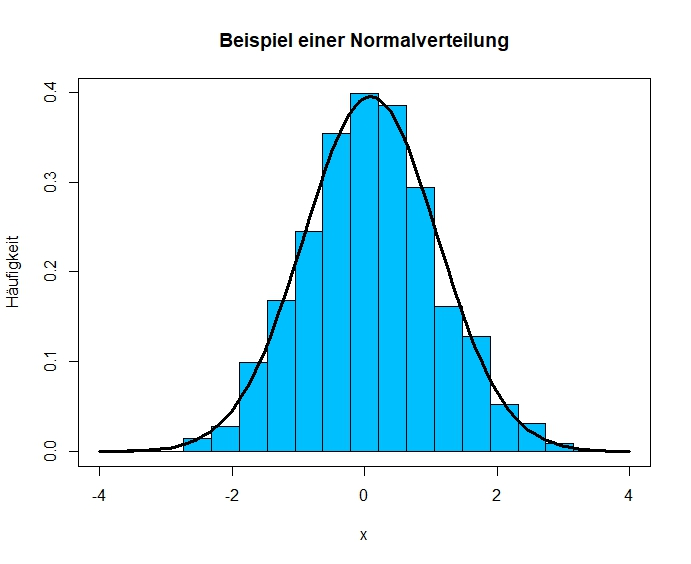
\includegraphics{BeispielNormalverteilung.jpeg}
\caption{Ein mit R geplottetes Beispiel einer Normalverteilung}
\end{figure}

\section{Einstein-Smoluchowski-Gleichung}
\textbf{Was bedeuten die Größen in der Einstein-Smoluchowski-Gleichung und wie kann die
Gleichung verstanden werden?}

Die Einstein-Smoluchowski-Gleichung beschreibt den Zusammenhang zwischen der Brownschen Bewegung und der thermischen Energie. Die thermische Energie der Flüssigkeit ist die Vorraussetzung dafür, dass Brownsche Molekülbewegung stattfinden kann. Die Bewegungsenergie ist gleich der thermischen Energie und setzt sich aus Diffusion und Reibung der Teilchen in der Flüssigkeit zusammen. Sie ist folgendermaßen definiert:
\begin{equation}
DC=k_BT
\end{equation}

\noindent $D$=Diffusionskonstante\\
\noindent $C$=Stokessche Reibungskonstante\\
\noindent $k_B$ = Boltzmann-Konstante\\
\noindent $T$ = Temperatur [K]\\

Die Reibungskonstante $C$ gibt dabei an, wie stark die Reibung auf eine Kugel mit dem Radius $r$ in einer Flüssigkeit der Viskosität $\eta$ wirkt. 

\begin{equation}
C = 6\pi\eta r
\end{equation}

Die Diffusionskonstante wird aus der Gleichung für die Konzentration, abgeleitet nach der Zeit $t$, ermittelt:
\begin{equation}
\frac{\delta c}{\delta t}(x,t) = D \frac{\delta^2 c}{\delta x^2}(x,t)
\end{equation}

\section{Diffusionskonstante}
\textbf{Was bedeuten die Größen in der Gleichung für die Diffusionskonstante und wie kann die Gleichung verstanden werden}

\begin{equation}
D= \frac{\sigma^2}{2t}
\end{equation}

\noindent $\sigma =$ Standardabweichung\\
Sie beschreibt, wie weit sich das Teilchen durchschnittlich in einer vorgebenen Zeit $t$ vom Ursprungspunkt entfernt. Dabei wird die Schrittweite des \textit{random walks} $\delta$ der mittleren Verschiebung angeglichen. Dieses entspricht dann genau der Standardabweichung.

\noindent $t =$ Zeit.

\end{document}